% !TeX root = ../main.tex
\chapter{特征点的提取与匹配}
\section{图像特征介绍}
图像匹配技术是计算机视觉领域的技术重要组成之一。图像匹配这项技术主要应用于目标识别、图像拼接、自动跟踪定位等研究。而基于特征点的图像匹配则是一种十分有效的方法。进行特征匹配的话,一般分为三个步骤,特征提取、特征描述和特征匹配。具体就是通过检测关键点,然后提取描述向量,最后来建立局部特征描述子,再进行特征匹配的过程。
\section{特征检测子}
\subsection{Harris 角点检测}
角点往往是两条边缘的交点,它是两条边缘方向变换的一种表示,因此其两个方向的梯度变换通常都比较大并且容易检测到。这里我们理解一下角点检测的算法。\par
\subsubsection{角点检测基本原理:}\par
人们通常通过在一个小的窗口区域内观察点的灰度值大小来识别角点,如果往任何方向移动窗口都会引起比较大的灰度变换那么往往这就是我们要找的角点。如下图:\par
\begin{figure}[htbp]
\centering
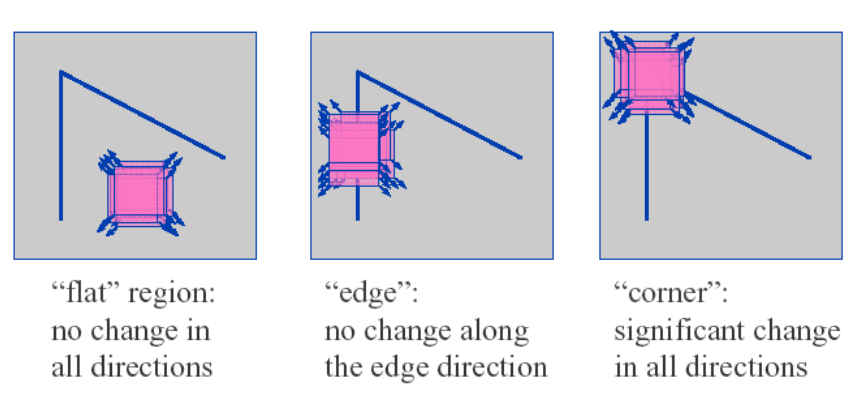
\includegraphics[height=5cm]{figures/Harris1.png}
\caption{角点的选择}
\end{figure}
\subsubsection{角点检测基本流程}
使用角点检测算子,对图像的每个像素计算角点响应函数(Corner Response Function ),阈值化角点响应函数,根据实际情况选择阈值,对阈值化的角点响应函数进行非极大值抑制,并获取非零点作为角点。
\subsubsection{Harris角点\cite{harris1988combined}}
下面我们看一下Harris的数学公式:
\begin{equation}
E(u,v)=\sum_{x}\sum_{y} w(x,y)[I(x+u,y+v)-I(x,y)]^{2}\label{Harris}
\end{equation}\par
式中$E(u,v)$即为角点响应函数,事实上被叫做窗口响应函数可能更合适,因为实际上$E(u,v)$计算的是一个5\times5或者7\times7的窗口。$x,y$为要计算的像素点。$I(x,y)$为该点的灰度值。$w(x,y)$为窗函数,可以理解为每个像素点的加权系数。
\begin{figure}[htbp]
	\centering
	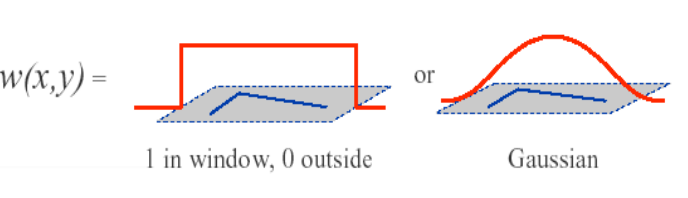
\includegraphics[height=3cm]{figures/Harris2.png}
	\caption{窗口函数}
\end{figure}
可以想象的到,对于平滑的,灰度值相对稳定的区域,该响应函数趋近于0;对于边缘区域,该响应函数在垂直于边缘方向上响应大,平行于边缘区域响应小;对于角点区域,无论什么方向响应都很大。道理是这个道理,但是给定上面的式子,变化u,v时,我们不能很直观的看出$E(u,v)$的变化。所以,我们要对上式进行一些变化和近似。使用泰勒级数展开,并忽略非线性项:
\begin{equation}
\begin{aligned}
I(x+u, y+v) &\approx I(x, y)+u I_{x}+v I_{y}+\omicron\left(I_x^{2},I_y^{2}\right)\\
&=I(x, y)+u I_{x}+v I_{y}
\end{aligned}
\end{equation}\par
由于图像的检测算子都很小,对上式做泰勒一阶展开是合理的,故响应函数可化为:
\begin{equation}
\begin{aligned}
E(u,v)=&\sum_{x,y} w(x,y) [I(x+u, y+v)-I(x, y)]^{2} \\
\approx&\sum_{x,y}w(x,y)\left[I(x, y)+u I_{x}+v I_{y}-I(x, y)\right]^{2}\\
=&\sum_{x,y}w(x,y) \left(u^{2} I_{x}^{2}+2 u v I_{x} I_{y}+v^{2} I_{y}^{2} \right)\\
=&\sum_{x,y}w(x,y) \left[ \begin{array}{cc}{u} & {v}\end{array}\right] \left[ \begin{array}{cc}{I_{x}^{2}} & {I_{x} I_{y}} \\ 
{I_{x} I_{y}} & {I_{y}^{2}}\end{array}\right] \left[ \begin{array}{c}{u} \\ 
{v}\end{array}\right]\\
=&\left[ \begin{array}{cc}{u} & {v}\end{array}\right]M\left[\begin{array}{c}{u}\\{v}\end{array}\right]
\end{aligned}
\end{equation}
其中:
\begin{equation}
M=\sum_{x, y} w(x, y) \left( \begin{array}{cc}{I_{x}^{2}} & {I_{x} I_{y}} \\ {I_{x} I_{y}} & {I_{y}^{2}}\end{array}\right)=\left( \begin{array}{cc}{\sum_{W} I_{x}^{2}} & {\sum_{W} I_{x} I_{y}} \\ {\sum_{W} I_{x} I_{y}} & {\sum_{W} I_{y}^{2}}\end{array}\right)=\left[ \begin{array}{cc}{A} & {C} \\ {C} & {B}\end{array}\right]
\end{equation}
故:
\begin{equation}
	E(u,v) \approx Au^{2}+2Cuv+Bv^{2}
\end{equation}
由公式\ref{Harris}可以看到,这样的函数在三维空间上起码是非负定的,如图\ref{ercixing}所示:
\begin{figure}[htbp]
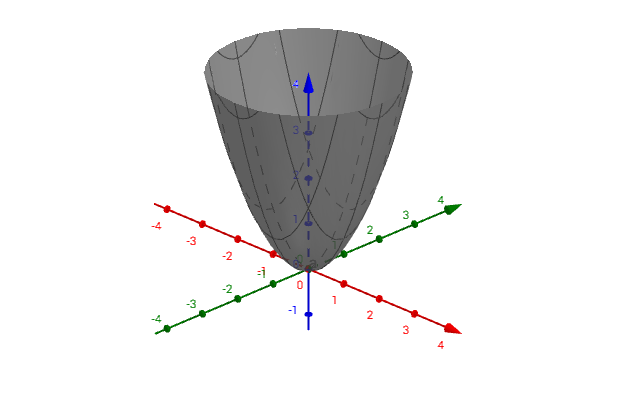
\includegraphics[height=5cm]{figures/ercixing.png}
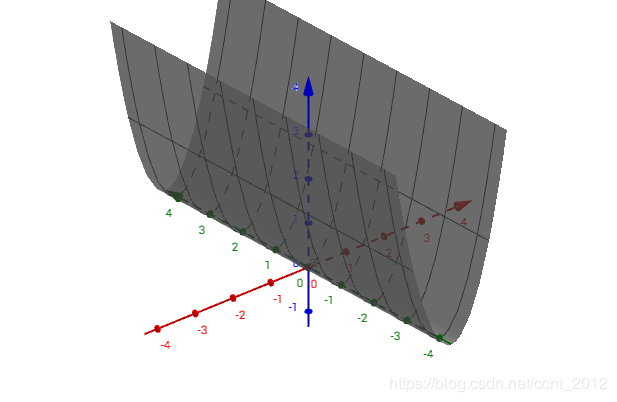
\includegraphics[height=5cm]{figures/ercixing1.png}
\caption{$E(u,v)$图像}
\label{ercixing}
\end{figure}\\
因此问题就变成了究竟怎样形式的E(u,v)的图像,才能算作一个特征点。直观上讲,一个角点应该无论在哪个方向上,响应函数$E$都应有一个大的变化。我们的也可以这么说:为了使响应函数$E$在角点邻域内有较大的变化量,M应该有两个较大的特征值。论文\cite{harris1988combined}指出,二次型矩阵的两个特征值$\lambda_1$和$\lambda_2$与点邻域的性质有如下关系:
\begin{itemize}
	\item 若$\lambda_1 \approx 0$,$\lambda_2\approx 0$,则表示图像在此处变化不大;
	
	\item 若$\lambda_1 \approx 0$且$\lambda_2$具有很大的正值,则表示检测到了边缘;
	
	\item 若$\lambda_1$,$\lambda_2$都很大,则表示检测到了角点;
\end{itemize}
但是实际在应用中,由于计算特征值比较慢,我们转而计算函数$R$来得到结果。其中$\kappa$是灵敏度系数,$\kappa$越小越敏感,一般来说$\kappa=0.04$。
\begin{equation}
	R = \lambda_1\lambda_2-\kappa(\lambda_1+\lambda_2)^2=det(M)-\kappa trace^2(M)
\end{equation}
因此,算法并不直接计算特征值,而是通过矩阵的行列式和迹来测量角点,从而大大提高了计算效率。\par
算法在计算完图像中的角点之后,图像上某些区域可能会出现角点十分密集的情况,这时候就要进行\textbf{非最大值抑制(Non-maximal Suppression)}。也就是说只保留局部区域中响应最大的特征点,从而避免匹配的时候重复检测。\par
\begin{figure}[htbp]
	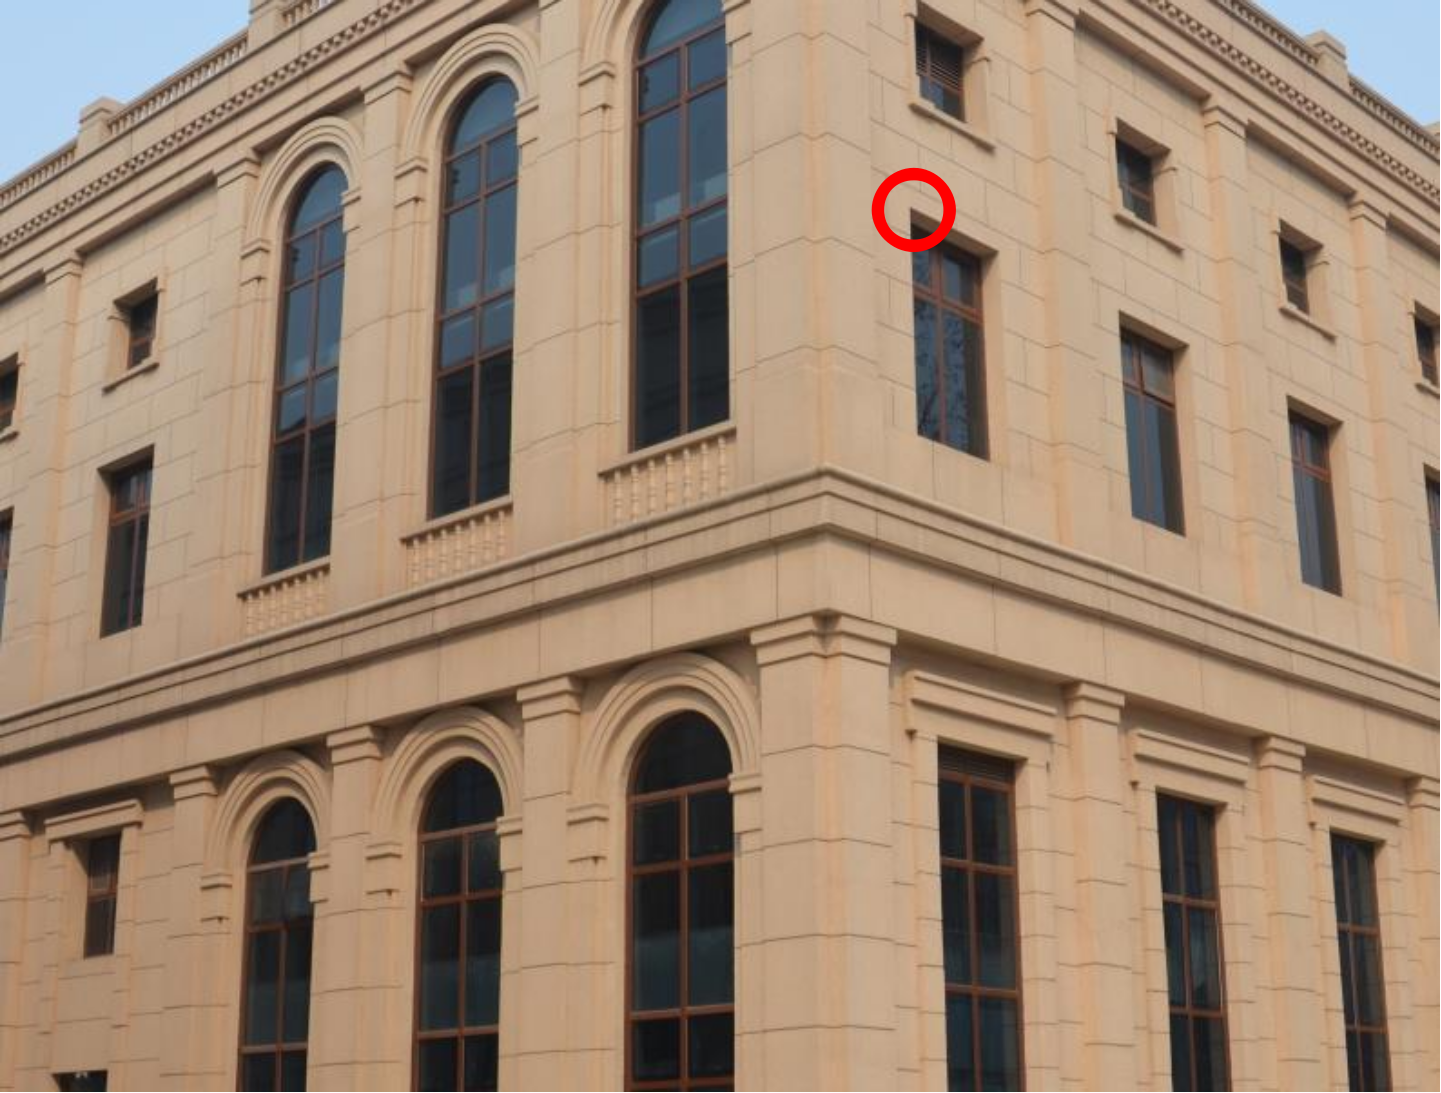
\includegraphics[height=5cm]{figures/LoG1.png}
	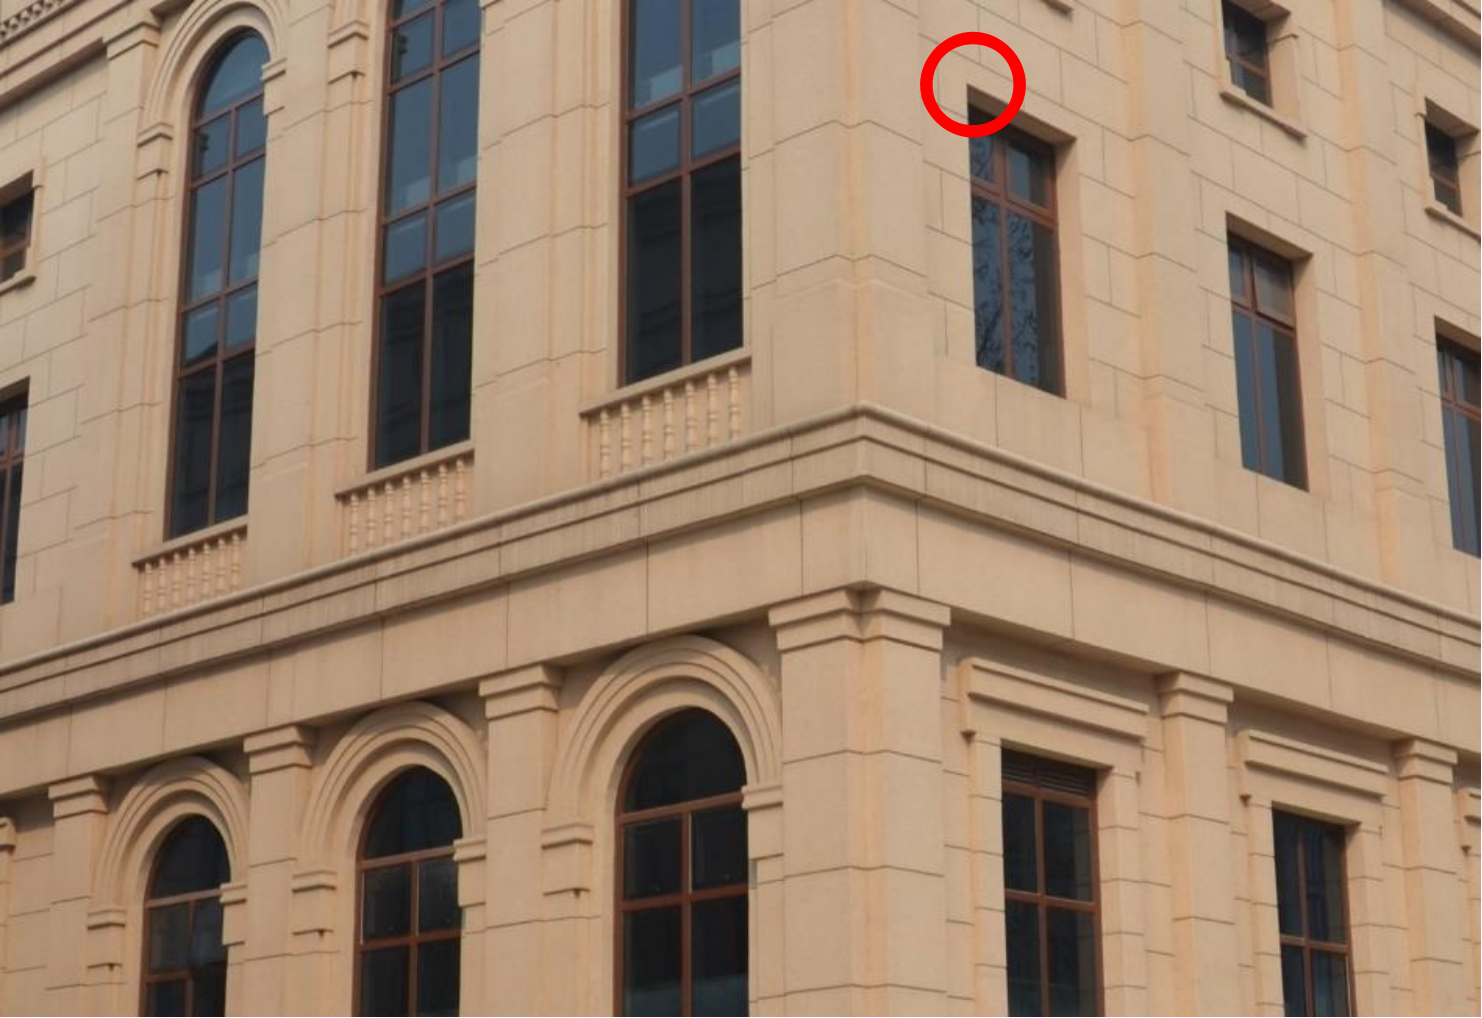
\includegraphics[height=5cm]{figures/LoG2.png}
	\caption{Harris角点不具有尺度不变性}
	\label{HarrisScale}
\end{figure}
这样,基于Harris角点的特征点检测方法已经介绍完了,但是这种角点并不完美。最大的问题就是Harris角点的检测窗口大小是固定的,也就是说Harris角点不具有尺度不变性。如图\ref{HarrisScale}可以看出来。左侧图像期望一个小的检测窗口,而右侧图像期待一个大的检测窗口。显然,在尺度变化较大的图像中,Harris角点并不能胜任检测工作,由此我们引出基于LoG的多尺度特征检测子。\par

\subsection{基于LoG的多尺度特征检测子}
\subsubsection{Laplace算子}
Laplace算子简单来说是两个梯度算子的点乘:
\begin{equation*}
\triangle=\nabla \cdot \nabla=\nabla^{2}=\left[\frac{\partial}{\partial x_{1}}, \cdots, \frac{\partial}{\partial x_{N}}\right] \left[ \begin{array}{c}{\frac{\partial}{\partial x_{1}}} \\ {\vdots} \\ {\frac{\partial}{\partial x_{N}}}\end{array}\right]=\sum_{n=1}^{N} \frac{\partial^{2}}{\partial x_{n}^{2}}
\end{equation*}
对于图像处理来说,一般用到的是二维的Laplace算子:
\begin{equation*}
\triangle=\nabla \cdot \nabla=\nabla^{2}=\left[\frac{\partial}{\partial x} \frac{\partial}{\partial y}\right] \left[ \begin{array}{c}{\frac{\partial}{\partial x}} \\ {\frac{\partial}{\partial y}}\end{array}\right]=\frac{\partial^{2}}{\partial x^{2}}+\frac{\partial^{2}}{\partial y^{2}}
\end{equation*}
对于函数$f(x,y)$应用Laplace算子:
\begin{equation*}
\triangle f(x, y)=\frac{\partial^{2} f}{\partial x^{2}}+\frac{\partial^{2} f}{\partial y^{2}}
\end{equation*}
对于离散的情况,二阶微分就变成了二阶差分。\par
我们先来看看在一维情况下将一阶差分:
\begin{equation*}
\nabla f[n]=f[n+1]-f[n]
\end{equation*}
那么一维的二阶差分就是:
\begin{equation*}
	\begin{aligned}
	\triangle f[n]=&\nabla(\nabla f[n])=\nabla f[n]-\nabla f[n-1]\\
	=&(f[n+1]-f[n])-(f[n]-f[n-1])\\
	=&f[n+1]-2 f[n]+f[n-1]
	\end{aligned}
\end{equation*}
因此,在一维情况下,Laplace算子可以理解成一维的卷积,其卷积核是$[1,-2,1]$。\par
在二维情况下,Laplace算子是两个维度中两个二阶差分的总和:
\begin{equation}
\begin{aligned}
\triangle f[m, n]=&\triangle_{m}[f[m, n]]+\triangle_{n}[f[m, n]]\\
=&f[m+1, n]-2 f[m, n]+f[m-1, n]+f[m, n+1]-2 f[m, n]+f[m, n-1]\\
=&f[m+1, n]+f[m-1, n]+f[m, n+1]+f[m, n-1]-4 f[m, n]
\end{aligned}
\end{equation}
此操作也可以理解成二维的卷积,其卷积核是:
\begin{equation*}
\left[ \begin{array}{lll}{0} & {1} & {0} \\ {1} & {-4} & {1} \\ {0} & {1} & {0}\end{array}\right]
\end{equation*}
\subsubsection{LoG算子}
图像中的噪声和边缘一样会使图像产生灰度跳变,我们在使用Laplace算子检测边缘细节的同时,往往也增强了噪声,因此,如何区分开噪声和边缘是个问题。\par
为了在取得较好的检测同时把噪声干扰降到最低,可以先对有噪声的原始图像进行平滑滤波,然后再进行锐化处理增强边缘和细节。基于这一思想,Marr和Hildreth\cite{marr1980theory}提出了把高斯平滑算子和拉普拉斯锐化算子结合起来的方法,称之为拉普拉斯-高斯(LoG)算子。\par
高斯平滑算子:
\begin{equation}
G_{\sigma}(x, y)=\frac{1}{\sqrt{2 \pi \sigma^{2}}} \exp \left(-\frac{x^{2}+y^{2}}{2 \sigma^{2}}\right)
\end{equation}\par
LoG算子:
\begin{equation}
\triangle\left[G_{\sigma}(x, y) * f(x, y)\right]=\left[\triangle G_{\sigma}(x, y)\right] * f(x, y)=L o G * f(x, y)
\\
\end{equation}
\begin{equation}
\begin{aligned}
L o G \triangleq& \triangle G_{\sigma}(x, y)=\frac{\partial^{2}}{\partial x^{2}} G_{\sigma}(x, y)+\frac{\partial^{2}}{\partial y^{2}} G_{\sigma}(x, y)\\
=&\frac{x^{2}+y^{2}-2 \sigma^{2}}{\sigma^{4}} \exp \left(-\frac{x^{2}+y^{2}}{2 \sigma^{2}}\right)
\end{aligned}
\end{equation}\par
画出LoG算子的空间形状:
\begin{figure}[H]
	\centering
	\begin{subfigure}[ht]{0.3\textwidth}
		\centering
		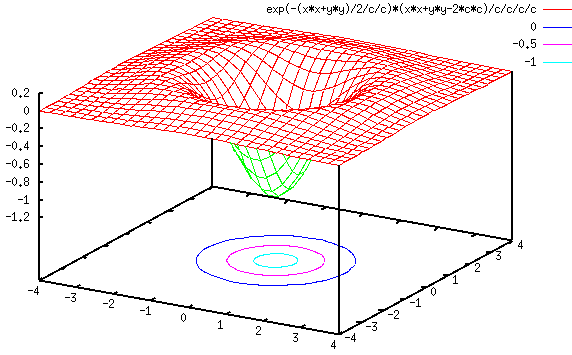
\includegraphics[height=0.7\textwidth]{figures/LoG_plot.png}
		\subcaption{连续空间表示}
	\end{subfigure}
\qquad \qquad \qquad
	\begin{subfigure}[ht]{0.3\textwidth}
		\centering
		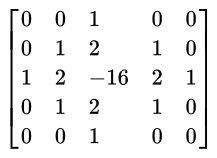
\includegraphics[height=0.7\textwidth]{figures/LoG_table}
		\subcaption{离散空间表示}
	\end{subfigure}
\caption{LoG算子空间表示}
\end{figure}
\begin{figure}[htbp]
\centering
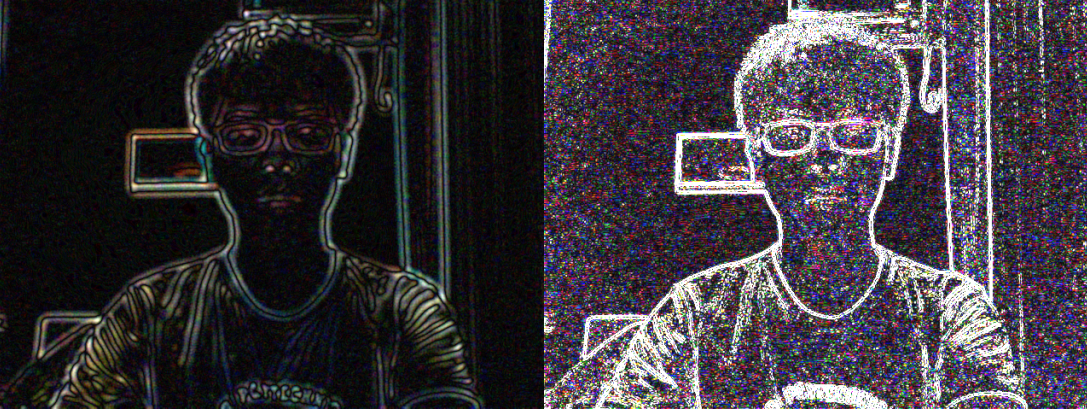
\includegraphics[height=3.5cm]{figures/LoG.png}
\caption{左:LoG算子\qquad \qquad \qquad \qquad 右:Laplace算子}
\end{figure}\par
可以看到,LoG算子显著减小了噪点对检测的影响。
\subsubsection{尺度空间}
为了解决一般角点不具有尺度不变性的问题,我们在此引入尺度空间:
\begin{equation}
L\left(x, y, \sigma_{D}\right)=I(x, y) * G\left(x, y, \sigma_{D}\right), \quad \sigma_{D} \in\left\{\sigma_{0}, \quad k \sigma_{0}, \quad k^{2} \sigma_{0}, \quad \dots\right\}
\end{equation}
尺度空间下的LoG算子:
\begin{equation}
\begin{aligned}
\nabla^{2} \mathrm{L}\left(x, y, \sigma_{\mathrm{D}}\right)=&\left(\frac{\partial^{2} \mathrm{L}\left(x, y, \sigma_{\mathrm{D}}\right)}{\partial x^{2}}+\frac{\partial^{2} \mathrm{L}\left(x, y, \sigma_{\mathrm{D}}\right)}{\partial y^{2}}\right)\\
=&\underbrace{\left(\frac{\partial^{2} \mathrm{G}\left(x, y, \sigma_{\mathrm{D}}\right)}{\partial x^{2}}+\frac{\partial^{2} \mathrm{G}\left(x, y, \sigma_{\mathrm{D}}\right)}{\partial y^{2}}\right)}_\text{多尺度LoG算子}*I(x,y)
\end{aligned}
\end{equation}
从公式可以看出,所谓尺度空间,就是用不同大小的高斯滤波核来对图像进行处理。如图\ref{differentkernalsize}所示:
\begin{figure}[H]
	\centering
	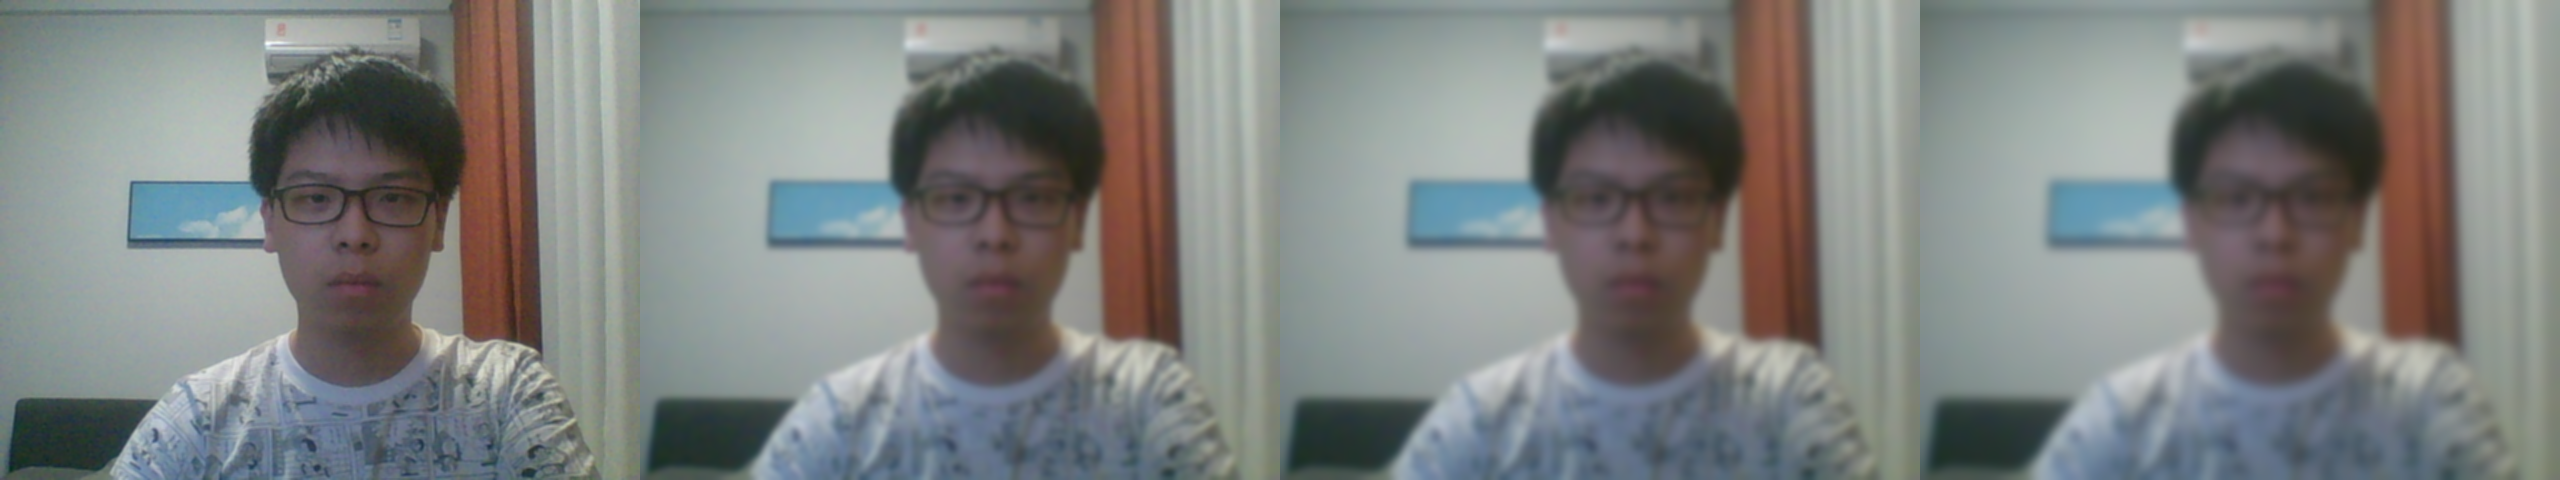
\includegraphics[height=3cm]{differentkernalsize.png}
	\caption{不同的高斯滤波核大小,从左至右依次是3$\times$3,11$\times$11,21$\times$21,25$\times$25}\label{differentkernalsize}
\end{figure}\par
可以看到滤波核越大,图像就越模糊。这实际上也是在模拟人类的视觉,因为距离越远,人看上去也越模糊。因此我们可以用不同滤波核来模拟不同的尺度。\par
但是这种多尺度的LoG算子有一个问题,不同尺度的LoG算子计算出来的响应值不具有可比性,因此我们需要对LoG算子进行归一化操作,才能够在不同尺度之间比较LoG算子的响应值,具体的做法就是将LoG算子乘上一个尺度:
\begin{equation}
\nabla_{\text { norm }}^{2} \mathrm{L}\left(x, y, \sigma_{\mathrm{D}}\right)= 
\underbrace{\sigma_{\mathrm{D}}^{2}\left(\frac{\partial^{2} \mathrm{G}\left(x, y, \sigma_{\mathrm{D}}\right)}{\partial x^{2}}+\frac{\partial^{2} \mathrm{G}\left(x, y, \sigma_{\mathrm{D}}\right)}{\partial y^{2}}\right)}_\text{尺度归一化LoG算子} * I(x, y)
\end{equation}
那么寻找特征点的过程,就可以转化为求解$| \nabla_{\text { nomm }}^{2} \mathbf{L}\left(x, y, \sigma_{\mathrm{D}}\right) |$最值的过程。\par
\subsection{基于DoG的多尺度特征检测子(sift}
实际上这种基于LoG算子检测特征点的方法效果是很好的,但是它十分耗费计算资源。计算速度不快。于是Lowe\cite{lowe2004sift}提出相邻尺度的高斯差分(DoG)来近似LoG算法,也就是所谓的sift特征点。Difference of Gaussian(DoG)是高斯函数的差分。字面意思理解,首先将图像与两个方差不同的高斯函数进行卷积得到两幅滤波结果,然后再将图像相减,得到DoG的响应值图像。
\begin{equation}
\begin{aligned} g_{1}(x, y) &=G_{\sigma_{1}}(x, y) * f(x, y) \\ g_{2}(x, y) &=G_{\sigma_{2}}(x, y) * f(x, y) \end{aligned}
\end{equation}
则DoG表示为:
\begin{equation}
D o G \triangleq G_{\sigma_{1}}-G_{\sigma_{2}}=\frac{1}{\sqrt{2 \pi}}\left(\frac{1}{\sigma_{1}} e^{-\left(x^{2}+y^{2}\right) / 2 \sigma_{1}^{2}}-\frac{1}{\sigma_{2}} e^{-\left(x^{2}+y^{2}\right) / 2 \sigma_{2}^{2}}\right)
\end{equation}
\begin{figure}[H]
	\centering
	\begin{subfigure}[ht]{0.3\textwidth}
		\centering
		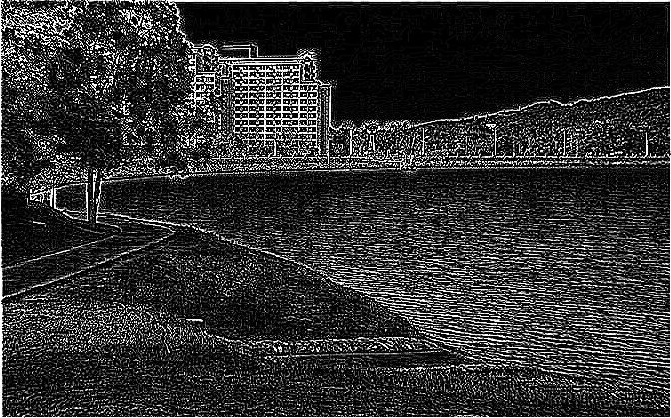
\includegraphics[height=0.7\textwidth]{figures/DoG1.png}
		\subcaption{$\sigma_1=$0.3,$\sigma_2=$0.4}
	\end{subfigure}
	\begin{subfigure}[ht]{0.3\textwidth}
		\centering
		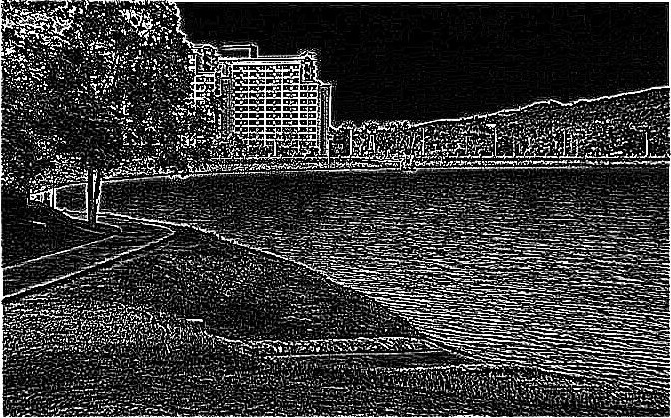
\includegraphics[height=0.7\textwidth]{figures/DoG2.png}
		\subcaption{$\sigma_1=$0.6,$\sigma_2=$0.7}
	\end{subfigure}
	\begin{subfigure}[ht]{0.3\textwidth}
	\centering
	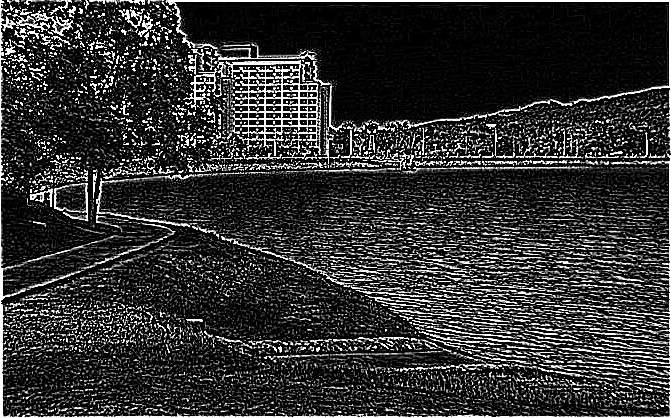
\includegraphics[height=0.7\textwidth]{figures/DoG3.png}
	\subcaption{$\sigma_1=$0.7,$\sigma_2=$0.8}
	\end{subfigure}
	\caption{不同高斯滤波函数相减}\label{differentsigma}
\end{figure}
根据理论,三维图中的最大值和最小值点是角点。在使用DoG求角点的时候,则采用多幅图像差分:\par
\begin{figure}[H]
	\centering
	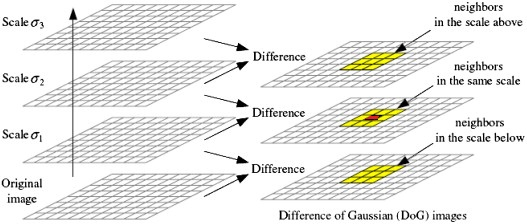
\includegraphics[height=5cm]{DoG.png}
	\caption{多尺度DoG}
\end{figure}\par
标记红色当前像素点,黄色的圈标记邻接像素点,用这个方式,最多检测相邻尺度的26个像素点。如果它是所有邻接像素点的最大值或最小值点,则标记红色被标记为特征点,如此依次进行,则可以完成图像的特征点提取。
因此根据图\ref{differentsigma},遍历图中每一个像素点,可以得到:
\begin{figure}[H]
	\centering
	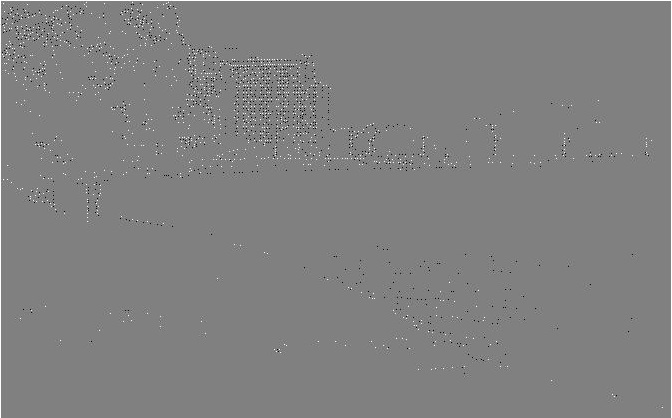
\includegraphics[height=5cm]{DoG4}
	\caption{黑色为极小值,白色为极大值}
\end{figure}\par
最后为了避免重复检测要进行非极大值抑制,把相邻的特征点进行删除,仅保留局部最大值。在原始图像上显示的DoG角点检测结果,如下图所示:
\begin{figure}
	\centering
	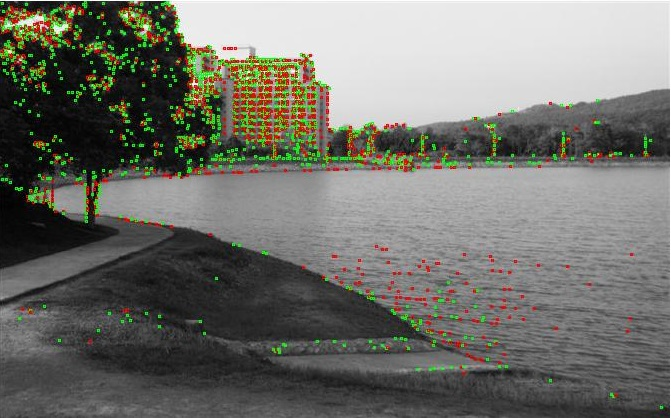
\includegraphics[height=5cm]{DoG5}
	\caption{DoG角点}
\end{figure}
\subsection{快速特征点检测方法}
\subsubsection{FAST特征点}
FAST特征点(Feature from Accelerate Segment Test)\cite{rosten2005fusing}是一种十分快速的特征点检测方法,速度是DoG的100倍。FAST特征点的检测方法很简单,就是检测局部像素灰度值变化来确认特征点的位置。\par
\begin{figure}[H]
	\centering
	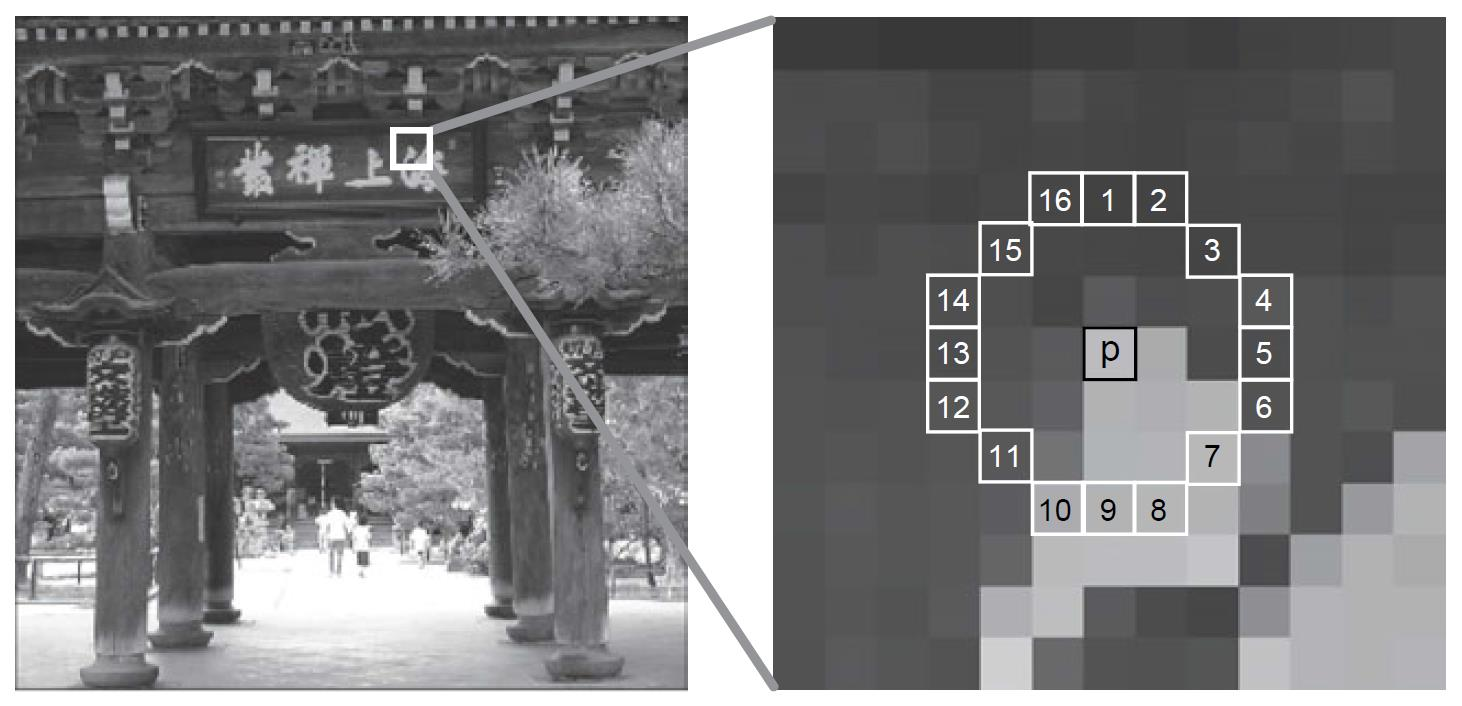
\includegraphics[height=5cm]{FAST}
	\caption{FAST检测原理}
\end{figure}
当有n个像素灰度值明显大于或者小于候选点的时候,该点被认为是特征点。\par
根据n的取值,这些特征点被叫做FAST-n特征点,n一般取9-12。
\subsubsection{ORB特征点}
ORB特征点(Oriented FAST),是用来弥补FAST特征点不具有尺度变性和旋转不变性而设计出来的特征点。事实上ORB特征点也是现阶段SLAM最经常使用的特征点。为了解决尺度不变性,我们可以构造多尺度的图像,在每一层上都进行检测。而对于旋转不变性,我们将在下一节从特征点描述子入手来解决旋转不变性的问题。
\section{特征描述子}
\subsection{描述子的要求}
上一节说明了如何去提取特征点,但是在图像处理过程中提取特征点之后还需要对特征点进行描述。特征描述子就好像是特征点的ID一样。即便在两幅图像中,如果两个特征点的描述子很接近,我们就有一定的把握说这两个特征点是现实空间中的同一个点。这就对描述子有以下几个要求:
\begin{itemize}
	\item 同一个空间点在不同视角的特征点具有高度相似的描述子
	\item 不同的描述子之间差异性应该尽量的大
	\item 描述子需要是一个具有固定长度的向量
	\item 一定的鲁棒性,在不同光照,不同角度下描述子应该相似
\end{itemize}
\subsection{支撑区域与主方向}
某个特征点的描述子计算需要有一个支撑区域,描述子就是根据这个支持区域来计算的。支持区域可以是正方形的,也可以是长方形的。对于较大的图片我们可以采用较大的支持区域,反之亦然。不同大小的支持区域实际上也反映了一个尺度的变化。\par
常见的例如BRIEF是一种二进制描述子,其描述向量由许多0和1组成,这里的0和1编码了关键点附近两个像素的大小关系。如果我们取了256组点,最后就得到了256维由0、1组成的向量。BRIEF是随机选点的,速度非常快,而且由于使用了二进制表达,存储也十分的方便。但是这样的描述子是不具有旋转不变性的,事实上,由于其极快的速度,目前许多SLAM系统中采用的就是添加了角度信息的BRIEF描述子。我们在计算描述子的同时,还通过特征点获得到了它的主方向,大概理解就是支撑区域中每个像素的梯度方向的一个加权和。主方向描述了支撑区域中大多数点的一个梯度方向。因此在计算描述子的时候,我们可以先将主方向旋转到水平方向,然后再进行计算,这样我们计算到的描述子就具有了旋转不变性。
\begin{figure}[H]
	\centering
	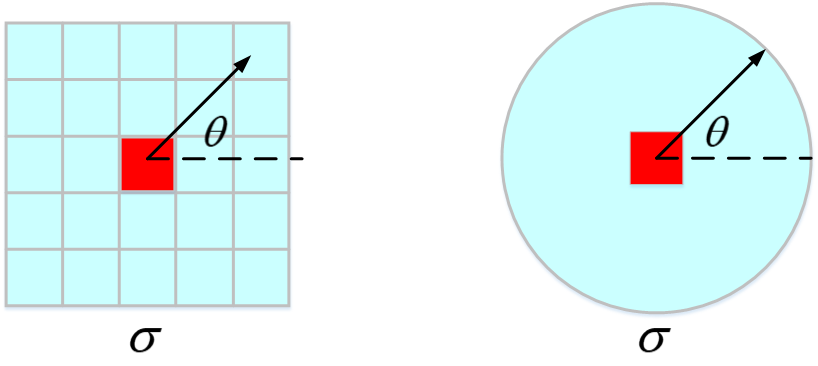
\includegraphics[height=5cm]{zhichiquyu}
	\caption{描述子支撑区域及主方向}
\end{figure}
\subsection{光度一致性}
为了让描述子在不同的光照条件下都有较好的表现,我们通过将图像像素值进行归一化处理,去除光度变化。
\begin{equation}
I^{\prime}=\frac{I-u}{s}
\end{equation}\par
为了解决尺度不变性,我们引入了支撑区域;为了解决旋转不变性,我们将图像主方向旋转至水平;为了解决光照一致性,我们将图像归一化。经过这几个步骤,我们就能过获得一个良好的描述子了。表\ref{descriptors}列出了几种常见的描述子。
\begin{table}[htbp]
	\caption{常见描述子}
	\label{descriptors}
	\begin{tabular}{p{0.16\textwidth}<{\centering} p{0.28\textwidth}<{\centering} p{0.28\textwidth}<{\centering} p{0.28\textwidth}<{\centering}}
		\toprule
		\multicolumn{1}{c}{} & SIFT                                         & SURF                                              & BRIEF                                                \\ \midrule
		确定主方向                & 支撑区域梯度直方图最值方向                                & 支撑区域对Haar算子响应最大方向                                 & 无                                                    \\ \midrule
		确定尺度                 & 建立尺度空间,尺度空间中DoG最值所在的尺度即为特征尺度                 & 尺度空间中Hessian矩阵行列式最值所在的尺度即为特征尺度                    & 无                                                    \\ \midrule
		描述方法                 & 取一正方形支撑区域,分为4×4个子区域,每个区域用8方向的梯度表示每个子区域,共128维 & 同样取4×4个子区域,分别在x,y方向计算Haar算子响应值之和和绝对值之和,4个值描述,共64维 & 在特征点周围随机抽取点对并灰度值大小,根据结果记作0或1,取256组组成256位的二进制串 \\ \bottomrule
	\end{tabular}
\end{table}
\section{特征点匹配}
考虑这样一个问题:对于一个场景,我们在两个不同的角度进行拍摄得到两张照片。对这两张照片提取特征点之后如何去判断哪两个特征点描述的是空间中的同一个点呢?这就引出了特征点匹配问题。前面说了,特征点的描述子就像特征点的ID一样,我们希望不管这个点在什么条件下,总是能被人们检测出这就是那个点。我们可以这样认为:一个设计良好的描述子,它在不同视角下的距离应该是差不多的。\par
\begin{figure}[H]
	\centering
	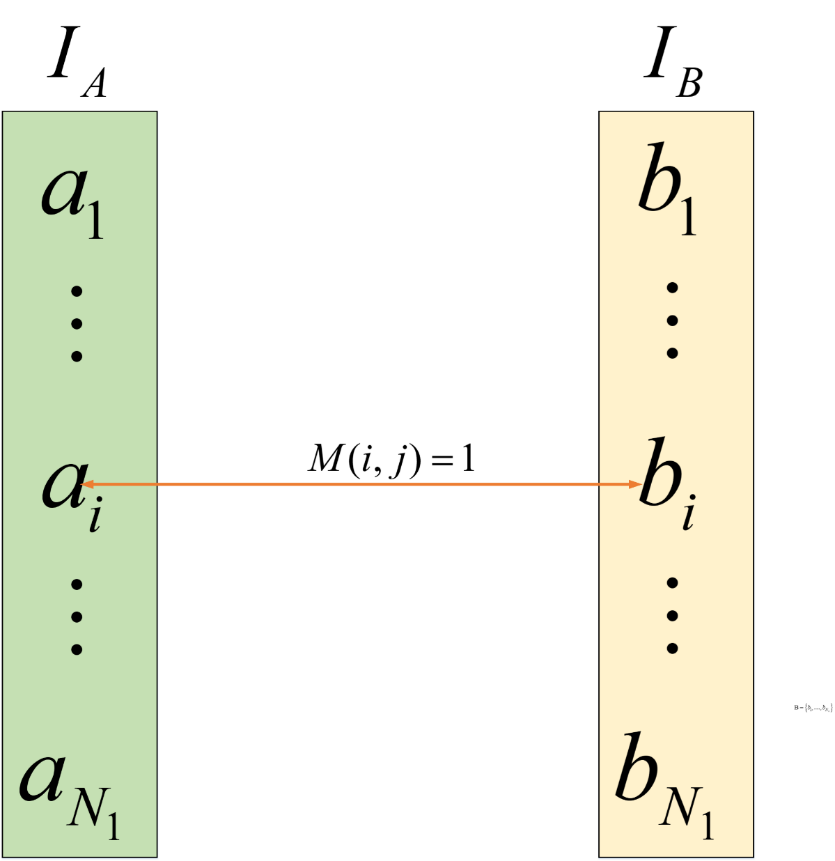
\includegraphics[height=5cm]{tezhengdianjuli}
	\caption{特征点A和B的描述子}
\end{figure}
我们有很多种方法可以度量两个描述子是否接近:
\begin{table}[htb]
	\centering
	\caption{度量距离的几种方法}
	\begin{tabular}{ll}
		\toprule
		距离 & 公式\\
		\midrule
		欧式距离 & $D_{e u c}(\boldsymbol{a}, \boldsymbol{b})=\|\boldsymbol{a}-\boldsymbol{b}\|_{2}=\left(\sum_{i=1}^{n}\left(a_{i}-b_{i}\right)^{2}\right)^{\frac{1}{2}}$ \\
		马氏距离 & $D_{\text {mahal}}(\boldsymbol{a}, \boldsymbol{b})=\left((\boldsymbol{a}-\boldsymbol{b})^{T} \Sigma^{-1}(\boldsymbol{a}-\boldsymbol{b})\right)^{\frac{1}{2}}$   \\
		归一化互相关 & $N C C(\boldsymbol{a}, \boldsymbol{b})=\sum_{i=1}^{n} \frac{1}{s_{a} s_{b}}\left(a_{i}-u_{a}\right)\left(b_{i}-u_{b}\right)$       \\
		汉明距离 & $D_{h a m}(\boldsymbol{a}, \boldsymbol{b})=\sum_{i=1}^{n} a_{i} \oplus b_{i}$\\
		\bottomrule	
	\end{tabular}
  \note{注:$a_{i} \oplus b_{i}$即两者相同时为1,不同为0}
\end{table}
\subsection{匹配策略}
特征的匹配是针对特征描述子的进行的,上面提到特征描述子通常是一个向量,两个特征描述子的之间的距离可以反应出其相似的程度,也就是这两个特征点是不是同一个。根据描述子的不同,可以选择不同的距离度量。如果是浮点类型的描述子,可以使用其欧式距离;对于二进制的描述子(BRIEF)可以使用其汉明距离。\par
\subsubsection{Lowe’s algorithm}
有了计算描述子相似度的方法,那么在特征点的集合中如何寻找和其最相似的特征点,这就是特征点的匹配了。最简单直观的方法就是暴力匹配方法(Brute-Force Matcher),计算某一个特征点描述子与其他所有特征点描述子之间的距离。
\begin{figure}[H]
\centering
\begin{subfigure}[ht]{0.4\textwidth}
	\centering
	\includegraphics[height=4cm]{matches}
	\caption{BFMatcher结果}
\end{subfigure}
\quad
\begin{subfigure}[ht]{0.4\textwidth}
	\centering
	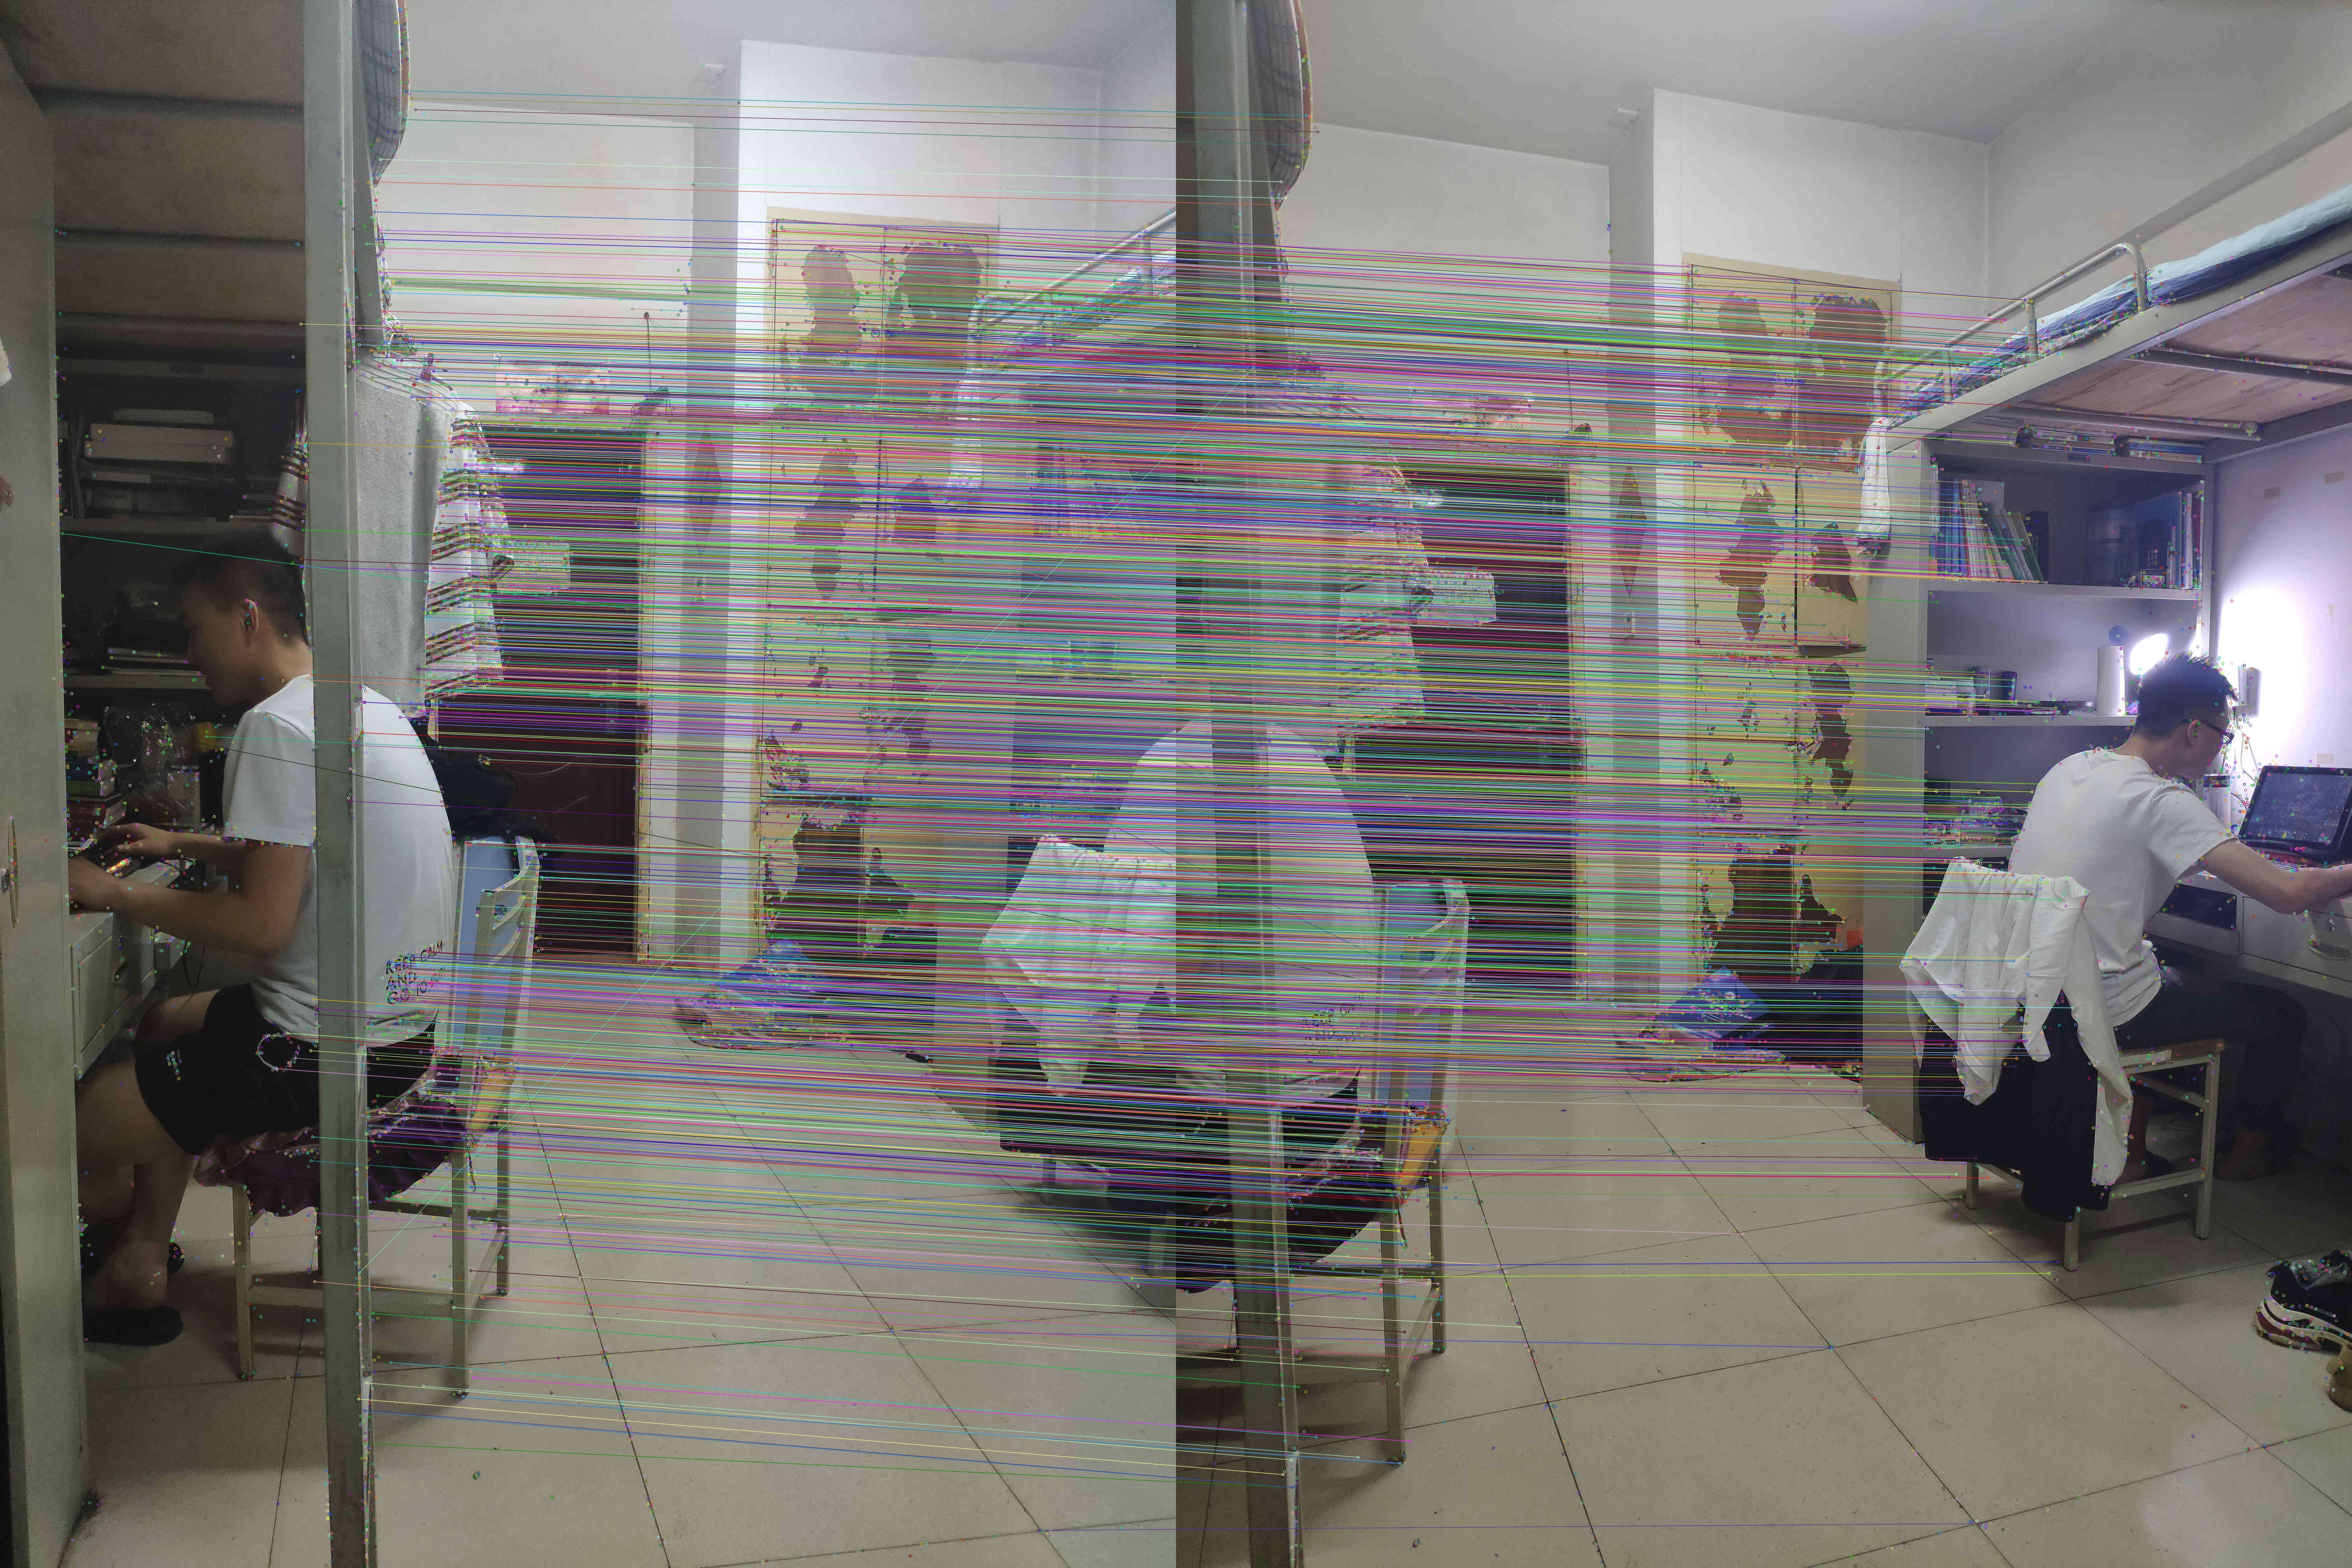
\includegraphics[height=4cm]{matches1}
	\subcaption{Lowe‘s算法过滤}
	\label{lowe's filter}
\end{subfigure}
\caption{匹配过程}\label{differentsigma}
\end{figure}
然后将得到的距离进行排序,取距离最近的一个作为匹配点。这种方法简单粗暴,其结果也是显而易见的,通过上面的匹配结果,也可以看出有大量的错误匹配,这就需要使用一些机制来过滤掉错误的匹配。\par
Lowe's algorithm\cite{muja2009fast}是我们常用的过滤掉错误匹配点的方法。它的原理也很简单,对于一幅图中的特征点,找到另一幅图中和它欧氏距离最近的两个特征点,如果最邻近距离除以次临近距离的值小于某个阈值,则说明最邻近点相比于次临近点足够优秀,就认为这一对点是一组匹配,反之则不是。如图\ref{lowe's filter}所示,可以显然看到经过过滤之后匹配的点已经很准确了。
\subsubsection{交叉匹配}
交叉过滤基于这样一个简单的设想:如果特征点A认为B是它的最优匹配,那么相应的,特征点B也应该认为特征点A是它的最优匹配。具体操作的话就是再进行一次匹配,反过来使用被匹配到的点进行匹配,如果匹配到的仍然是第一次匹配的点的话,就认为这是一个正确的匹配。假如第一次特征点A使用暴力匹配的方法匹配到特征点B;反过来,使用特征点B进行匹配,如果匹配到的仍然是特征点A,则就认为这是一个正确的匹配,否则就是一个错误的匹配。














